\subsection{BOREL SETS}

DEFINITION 3. Let X be a set and let \(\mathfrak{X}\) be a set of subsets of X. \(\mathfrak{X}\) is said to be a \(\sigma\) -algebra on X if the following conditions are satisfied:

\begin{enumerate}
\def\labelenumi{\alph{enumi})}
\item
  The complement of every set of \(\mathfrak{S}\) belongs to \(\mathfrak{S}\) .
\item
  Every countable intersection of sets of \(\mathfrak{X}\) belongs to \(\mathfrak{X}\) .
\end{enumerate}

If \(\mathfrak{X}\) is a \(\sigma\) -algebra on \(\mathbf{X}\) , every countable union of sets of \(\mathfrak{X}\) belongs to \(\mathfrak{X}\) (for the complement of this union is an intersection of sets of \(\mathfrak{X}\) ).

The set \(\mathfrak{P}(\mathbf{X})\) of all subsets of X is clearly a \(\sigma\) -algebra. Every intersection of \(\sigma\) -algebras on X is a \(\sigma\) -algebra on X. For any subset of \(\mathfrak{P}(\mathbf{X})\) , there is therefore a smallest \(\sigma\) -algebra containing F; it is called the \(\sigma\) -algebra generated by F.

DEFINITION 4. In a topological space X, the elements of the \(\sigma\) -algebra generated by the set of all closed subsets of X are called Borel sets in X.

PROPOSITION 10. Let \(f\) be a continuous mapping of a topological space \(\mathbf{X}\) into a topological space \(\mathbf{Y}\) . Then the inverse image under \(f\) of every Borel set in \(\mathbf{Y}\) is a Borel set in \(\mathbf{X}\) .

Let \(\mathfrak{X}\) be the set of all subsets \(\mathbf{A}\) of \(\mathbf{Y}\) such that \(\overline{f}^1 (\mathbf{A})\) is a Borel set in \(\mathbf{X}\) . It follows immediately that \(\mathfrak{X}\) is a \(\sigma\) -algebra which contains all the closed subsets of \(\mathbf{Y}\) ; hence \(\mathfrak{X}\) contains all Borel sets in \(\mathbf{Y}\) .

PROPOSITION II. In a Souslin space X, every Borel set is a Souslin set.

Let \(\mathfrak{X}\) be the set of all subsets A of X such that both A and CA are Souslin sets. By Proposition 8 of no. 2, \(\mathfrak{X}\) is a \(\sigma\) -algebra. Every closed subset F of X belongs to \(\mathfrak{X}\) , for both F and CF are Souslin sets (no. 2, Proposition 5); hence \(\mathfrak{X}\) contains all Borel sets of X (cf.~no. 6, Theorem 2, Corollary).

COROLLARY. Let \(f\) be a continuous mapping of a Souslin space \(\mathbf{X}\) into a metrizable space \(\mathbf{Y}\) . If \(\mathbf{B}\) is any Borel set in \(\mathbf{X}\) , then \(f(\mathbf{B})\) is a Souslin set in \(\mathbf{Y}\) .

For B is a Souslin space, hence so is \(f(\mathbf{B})\) by the remark following Definition 2 (no. 2).

\pandocbounded{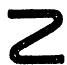
\includegraphics[keepaspectratio]{images/part002_bde2d1b5.jpg}}

Remarks. 1) Even when X and Y are Polish spaces it is not in general true that the image of a Borel set in X under a continuous mapping of X into Y is a Borel set in Y (cf.~Exercise 6; and no. 7, Theorem 3 Corollary).

\begin{enumerate}
\def\labelenumi{\arabic{enumi})}
\setcounter{enumi}{1}
\tightlist
\item
  Let X be a topological space and let Y be a Borel subset of X. Then the Borel sets of the space Y are exactly the Borel sets of X which are contained in Y. For (i) the Borel sets in X which are contained in Y form a σ-algebra on Y which contains the closed sets in Y and hence contains all Borel sets of Y; (ii) the subsets A of X such that A∩Y is a Borel set of Y form a σ-algebra on X which contains all the closed sets of X and therefore contains all Borel sets of X.
\end{enumerate}

